%\documentclass{article}
\documentclass[a4paper, 11pt]{article}
\usepackage{color}
\usepackage{eurosym}
\usepackage{graphicx}
\usepackage{subfigure}
\newcommand{\beq}{\begin{equation}}
\newcommand{\eeq}{\end{equation}}
\newcommand{\bef}{\begin{figure}}
\newcommand{\enf}{\end{figure}}
\newcommand{\p}{\partial}
\newcommand{\f}{\frac}
\newcommand{\ig}{\includegraphics}
\usepackage[margin={2.5cm, 2.5cm, 2.5cm, 2.5cm}]{geometry}
\usepackage{float}
%\floatstyle{boxed} 
\restylefloat{figure}


\begin{document}

\begin{center}
  {\Large \textbf{Shallow Water Equations for River Flows}}\\
   Seshu Tirupathi, IBM Research
\end{center}

Shallow water equations describing unsteady open channel flows are
typically used to model river flows. Conservative form of the
equations are difficult to numerically formulate and apply in real
test cases (Eq. $1$ in  \cite{garcia2008shallow}). On the other hand, the non conservative form of the equations are easier to formulate numerically (Eq. $3$ in \cite{garcia2008shallow}). There have been various attempts to handle both these formulations. It is important to note that the one dimensional model decreases the computational cost significantly to model river flows to a reasonable accuracy as compared to a more comprehensive 2D resolution. The problem becomes tricky when there is confluence of river segments/channels (Fig. 1). 
\begin{figure}[htb]
\centering
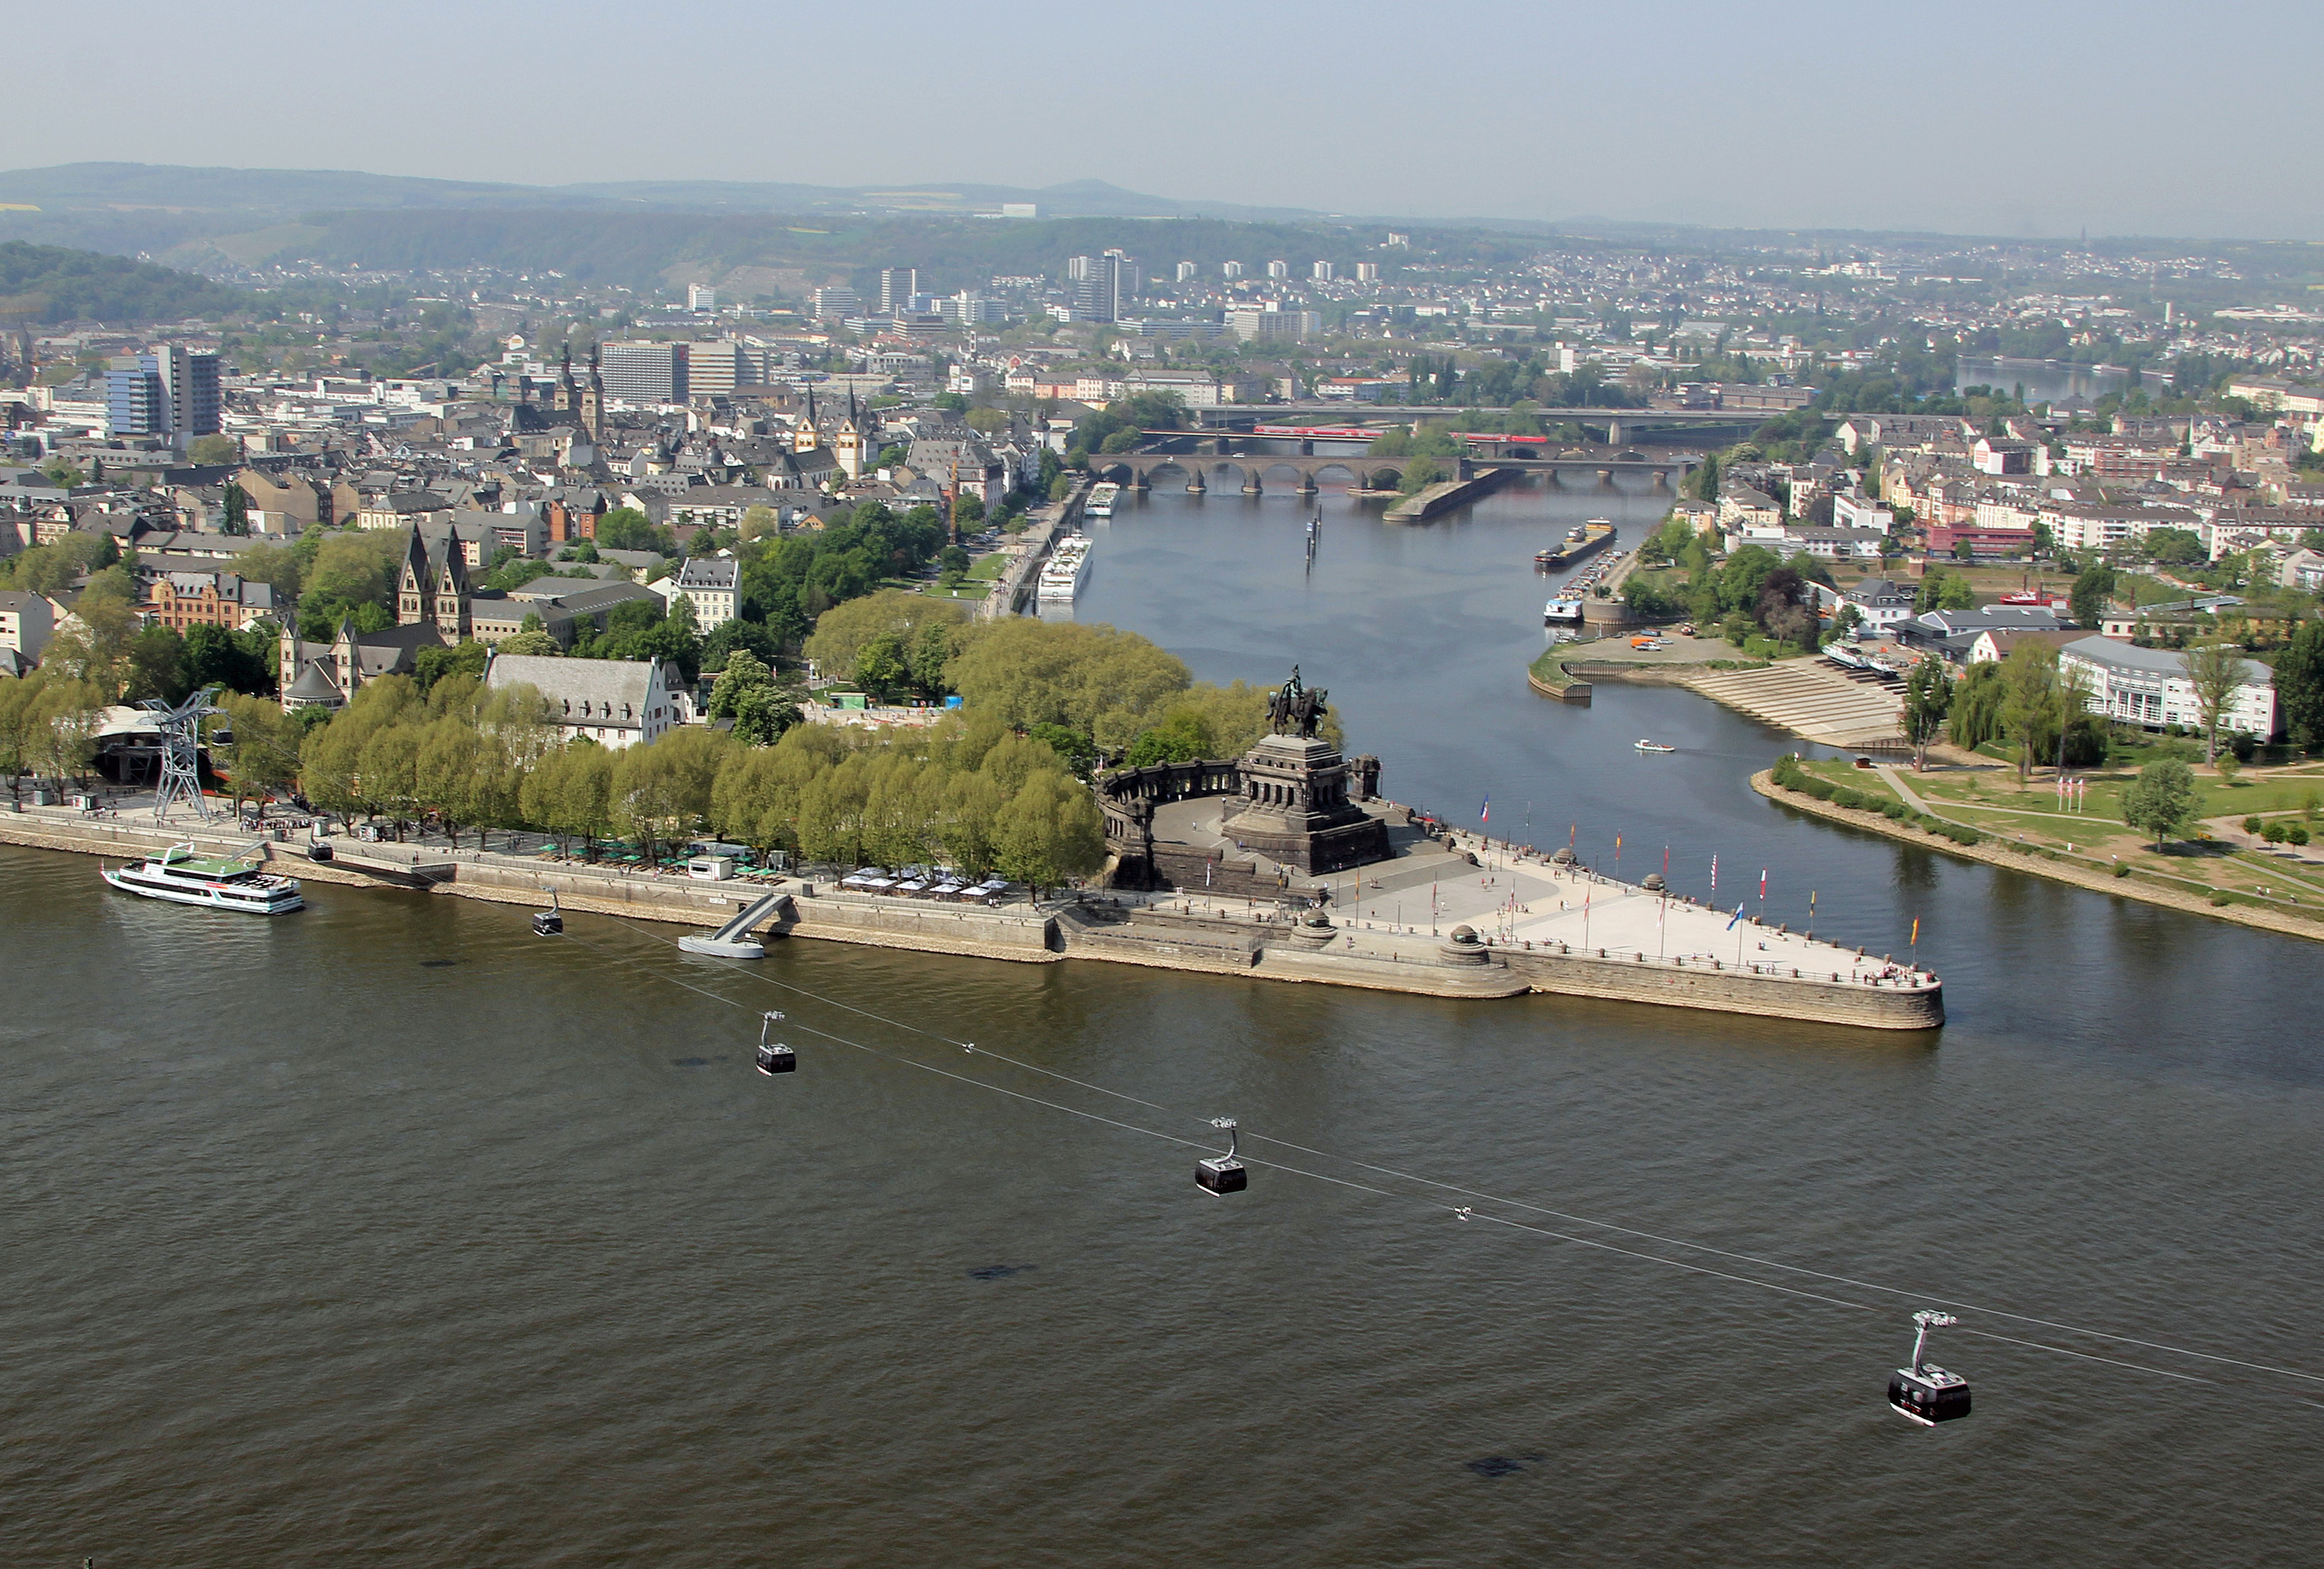
\includegraphics[width=0.6\linewidth]{./confluence}
\caption{Confluence of rivers, the Mosel flows into the Rhine at Koblenz (From wikipedia (By Holger Weinandt)) }
\end{figure}
Work has been done to handle merging of flows from different channels into a single channel by using a 2D formulation at the junction. 

For this workshop, can you comment on some or all of the following aspects (assuming continuous flow): 
\begin{enumerate}
\item In general, are there any disadvantages of using the non-conservative form of the equations even if the flow is continuous? 
\item For flow at a junction, is it possible to come up with internal boundary conditions/constraints without the necessity to solve the 2D shallow water equations? How do the boundary conditions compare with a 1D-2D coupling at the junction? (reference: Fig. 2)
\begin{figure}[htb]
\centering
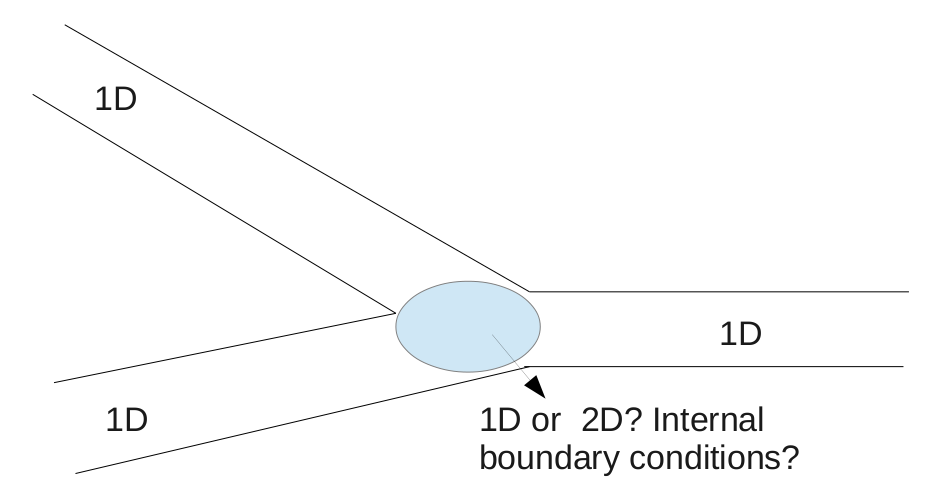
\includegraphics[width=0.5\linewidth]{./junction_1.png}
\caption{}
\end{figure}

\item How do the internal boundary conditions/constraints compare when the flow merges at a cross section? (reference: Fig. 3)
\begin{figure}
\centering
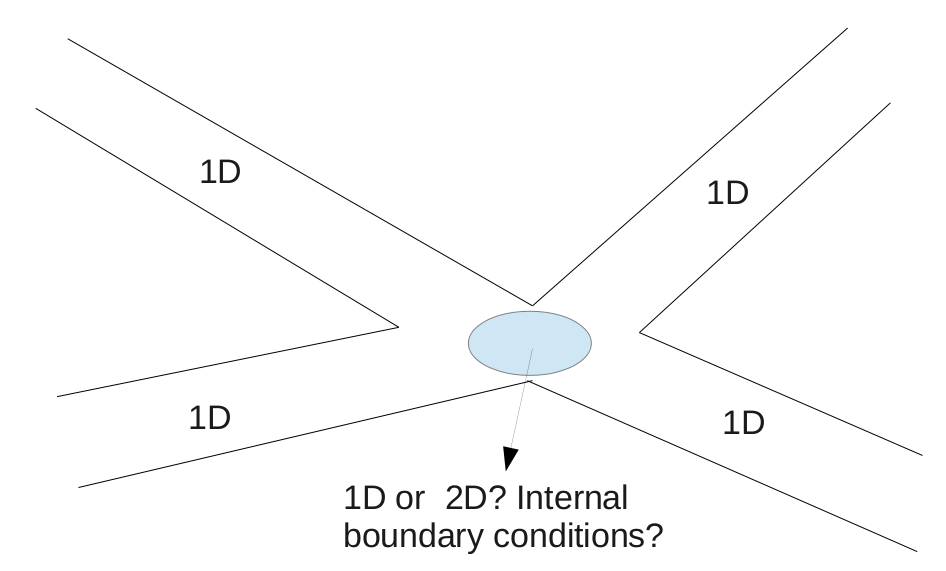
\includegraphics[width=.5\linewidth]{./junction_2.png}
\caption{}
\end{figure}
\item Can you come up with a rigorous analysis for questions $1-3$ assuming rectangular/trapezoidal/parabolic cross sections? 
\item What other novel methods can you come up with to handle merging flows while keeping the formulation limited to 1D?
\end{enumerate}






\bibliography{problem_statement}{}
\bibliographystyle{plain}

\end{document}

